\documentclass[conference]{IEEEtran}
\IEEEoverridecommandlockouts
% The preceding line is only needed to identify funding in the first footnote. If that is unneeded, please comment it out.
\usepackage{cite}
\usepackage{amsmath,amssymb,amsfonts}
\usepackage{algorithmic}
\usepackage{graphicx}
\usepackage{textcomp}
\usepackage{xcolor}
\usepackage{subfig}
\usepackage{float}

\def\BibTeX{{\rm B\kern-.05em{\sc i\kern-.025em b}\kern-.08em
    T\kern-.1667em\lower.7ex\hbox{E}\kern-.125emX}}
\begin{document}

\title{MO443 - Assignment I}

\author{210404 -- Guilherme Vieira Leite}

\maketitle

\section{Introduction}

In this work we explore some variants of the dithering technique and their effect on images. The implemented variant of dithering is the error

\section{Dithering Methods}
\label{sec:method}

The implemented dithering methods in this work differentiates between each other by a couple of factors: (i) whether they are grayscaled or colored, and (ii) the error diffusion matrix.

\paragraph{Color space} Dithering in the grayscale color space is performed as in the algorithm discussed in class, in a few words: the pixel is binarized, it's error is calculated and multiplied by the mask value relative to that pixel. To transfer this process to the RGB color space, we treated each of its three bands as if they were separate grayscale images, that were later combined together to create a dithered colored image.

\paragraph{Filter matrix} Each pixel is dithered by a error metric in relation to its neighbourhood, this neighbourhood is defined by the filter matrix, how large it is and which pixels are considered in the metric. In this work we tested on six pre-defined error diffusion matrices: Floyd and Steinberg, Stevenson and Arce, Burkes, Sierra, Stucki, and Jarvis, Judice, and Ninke, seen in Section~\ref{sec:appendix1}.

\section{Experiments}

Throughout our experiments we aimed to explore the effects of dithering, while varying the color space, the error diffusion matrix and the order in which the error was diffused. We also exchanged the output's quality by lower processing time, shrinking all input images to around 128x128, but the algorithm is still able to process larger images.

We performed dithering on {\color{red}nine} images, some provided by the professor and some particularly obtained. The images were chosen to exhaust the algorithm and explore its weaknesses and strengths, specially the colored dithering. Figure~\ref{fig:input} presents a few samples of the chosen images.

\begin{figure}[H]
\centering
\subfloat{
	{
		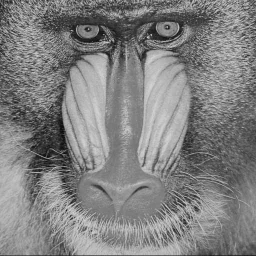
\includegraphics[scale=0.7]{figures/input/baboon}
	}
	\label{fig:baboon}
}
\subfloat{
	{
		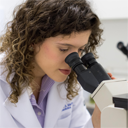
\includegraphics[scale=0.7]{figures/input/bee}
	}
	\label{fig:bee}
}
\quad
\subfloat{
	{
		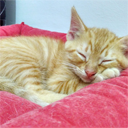
\includegraphics[scale=0.7]{figures/input/juquinha}
	}
	\label{fig:juquinha}
}
\subfloat{
	{
		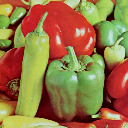
\includegraphics[scale=0.7]{figures/input/peppers}
	}
	\label{fig:peppers}
}
\quad
\subfloat{
	{
		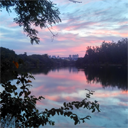
\includegraphics[scale=0.7]{figures/input/sky}
	}
	\label{fig:sky}
}
\subfloat{
	{
		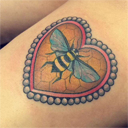
\includegraphics[scale=0.7]{figures/input/tattoo}
	}
	\label{fig:tattoo}
}
\caption{A sample of the images used in the experiments.}
\label{fig:input}
\end{figure}

We also experimented with three traversal methods, looping through the image from (i) left to right, top to bottom, (ii) right to left, bottom to top, and (iii) top to bottom, but every even row was looped left to right and every odd row was looped from right to left, seen in Figure~\ref{fig:traversal}. To traverse the images in these varying methods a few precautions had to be taken, since the chosen filters generates a particular effect, in which any pixel already dithered will be ignored to future error diffusion. We need to accommodate this effect on any traversal that differs from left to right, top to bottom, and we did so by tweaking with the filter's matrix to match the expected result, one example on Floyd and Steinberg can be seen in Table~\ref{tab:flo_inverse}.

\begin{figure}[H]
	\centering
	\subfloat{
		{
			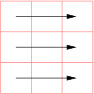
\includegraphics[scale=0.5]{figures/l2r}
		}
		\label{fig:l2r}
	}
	\quad
	\subfloat{
		{
			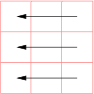
\includegraphics[scale=0.5]{figures/r2l}
		}
		\label{fig:r2l}
	}
	\quad
	\subfloat{
		{
			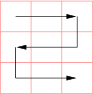
\includegraphics[scale=0.5]{figures/zz}
		}
		\label{fig:zz}
	}
	\caption{Traversal directions experimented on.}
	\label{fig:traversal}
\end{figure}

\begin{table}[H]
\centering
\renewcommand{\arraystretch}{1.5}
\begin{tabular}{c|c|c}
1/16 & 5/16             & 3/16 \\ \hline
7/16 & \textit{f(x, y)} &     
\end{tabular}
\caption{Floyd and Steinberg's diffusion error matrix when traversing from right to left, bottom to right.}
\label{tab:flo_inverse}
\end{table}

\section{Results}
\label{sec:results}

In this section we present and discuss the results obtained from the methods discussed in Section~\ref{sec:method}. To better explore the different aspects of a dithering process we focus our discussion on three subsections bellow.

\subsection{Color space}

In this experiment we performed a colored dithering and a grayscaled one. Although we are not exploring the effects of error diffusion and traversal direction, we also used Floyd and Steinberg's erro diffusion and traversed the image from left to right, top to bottom. Figure~\ref{fig:baboon_colorspace} shows the resulting dithering, in it we can observe that overall features of the image are kept, it is still possible to identify the baboon in frame, as it is the intention of dithering. But on a closer inspection it is also possible to notice a drop in quality of both images, also an expected effect, for instance the lower lip of the baboon has been filled with noise and mixes with the fur.

\begin{figure}[H]
	\centering
	\subfloat{
		{
			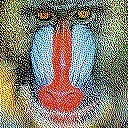
\includegraphics[scale=0.7]{figures/left2right/flo_color_baboon}
		}
		\label{fig:baboon_color}
	}
	\quad
	\subfloat{
		{
			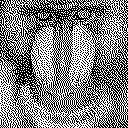
\includegraphics[scale=0.7]{figures/left2right/flo_gray_baboon}
		}
		\label{fig:baboon_gray}
	}
	\caption{Color and Grayscale dithering on Baboon.}
	\label{fig:baboon_colorspace}
\end{figure}

\subsection{Dithering matrices}

\begin{figure}[H]
	\centering
	\subfloat{
		{
			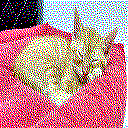
\includegraphics[scale=0.7]{figures/left2right/flo_color_juquinha}
		}
		\label{fig:flo_color_juquinha}
	}
	\subfloat{
		{
			\includegraphics[scale=0.7]{figures/left2right/ste_color_juquinha}
		}
		\label{fig:ste_color_juquinha}
	}
    \quad
	\subfloat{
		{
			\includegraphics[scale=0.7]{figures/left2right/bur_color_juquinha}
		}
		\label{fig:bur_color_juquinha}
	}
	\subfloat{
		{
			\includegraphics[scale=0.7]{figures/left2right/sie_color_juquinha}
		}
		\label{fig:sie_color_juquinha}
	}\quad
	\subfloat{
		{
			\includegraphics[scale=0.7]{figures/left2right/stu_color_juquinha}
		}
		\label{fig:stu_color_juquinha}
	}
	\subfloat{
		{
			\includegraphics[scale=0.7]{figures/left2right/jar_color_juquinha}
		}
		\label{fig:jar_color_juquinha}
	}
	\caption{Color Error Diffusion on Cat.}
	\label{fig:color_error_diffusion}
\end{figure}

\begin{figure}[H]
	\centering
	\subfloat{
		{
			\includegraphics[scale=0.7]{figures/left2right/flo_gray_juquinha}
		}
		\label{fig:flo_gray_juquinha}
	}
	\subfloat{
		{
			\includegraphics[scale=0.7]{figures/left2right/ste_gray_juquinha}
		}
		\label{fig:ste_cgray_juquinha}
	}
    \quad
	\subfloat{
		{
			\includegraphics[scale=0.7]{figures/left2right/bur_gray_juquinha}
		}
		\label{fig:bur_gray_juquinha}
	}
	\subfloat{
		{
			\includegraphics[scale=0.7]{figures/left2right/sie_gray_juquinha}
		}
		\label{fig:sie_gray_juquinha}
	}
	\quad
	\subfloat{
		{
			\includegraphics[scale=0.7]{figures/left2right/stu_gray_juquinha}
		}
		\label{fig:stu_gray_juquinha}
	}

	\subfloat{
		{
			\includegraphics[scale=0.7]{figures/left2right/jar_gray_juquinha}
		}
		\label{fig:jar_gray_juquinha}
	}
	\caption{Grayscale error diffusion on Cat.}
	\label{fig:gray_error_diffusion}
\end{figure}

\subsection{Traversal directions}

\begin{figure}[H]
	\centering
	\subfloat{
		{
			\includegraphics[scale=0.7]{figures/left2right/flo_color_bee}
		}
		\label{fig:l2r_flo_color_bee}
	}
	\subfloat{
		{
			\includegraphics[scale=0.7]{figures/right2left/flo_color_bee}
		}
		\label{fig:r2l_flo_color_bee}
	}
	\quad
	\subfloat{
		{
			\includegraphics[scale=0.7]{figures/zigzag/flo_color_bee}
		}
		\label{fig:zz_flo_color_bee}
	}
	\caption{Color traversal direction on Girl.}
	\label{fig:color_traversal_l2r}
\end{figure}

\begin{figure}[H]
	\centering
	\subfloat{
		{
			\includegraphics[scale=0.7]{figures/left2right/flo_gray_bee}
		}
		\label{fig:l2r_flo_gray_bee}
	}
	\subfloat{
		{
			\includegraphics[scale=0.7]{figures/right2left/flo_gray_bee}
		}
		\label{fig:r2l_flo_gray_bee}
	}
	\quad
	\subfloat{
		{
			\includegraphics[scale=0.7]{figures/zigzag/flo_gray_bee}
		}
		\label{fig:zz_flo_gray_bee}
	}
	\caption{Grayscale traversal direction on Girl.}
	\label{fig:gray_traversal_l2r}
\end{figure}

\subsection{Error function}


\section{Appendix I}
\label{sec:appendix1}

\begin{table}[!h]
\centering
\renewcommand{\arraystretch}{1.5}
\begin{tabular}{c|c|c}
     & \textit{f(x, y)} & 7/16 \\ \hline
3/16 & 5/16             & 1/16
\end{tabular}
\caption{Floyd and Steinberg's diffusion error matrix.}
\label{tab:flo}
\end{table}

\begin{table}[!h]
\centering
\renewcommand{\arraystretch}{1.5}
\begin{tabular}{c|c|c|c|c|c|c}
 & \textit{} &  & \textit{f(x, y)} &  & 32/200 &  \\ \hline
12/200 &  & 26/200 &  & 30/200 &  & 16/200 \\ \hline
 & 12/200 &  & 26/200 &  & 12/200 &  \\ \hline
5/200 &  & 12/200 &  & 12/200 &  & 5/200
\end{tabular}
\caption{Stevenson and Arce's diffusion error matrix.}
\label{tab:ste}
\end{table}

\begin{table}[!h]
\centering
\renewcommand{\arraystretch}{1.5}
\begin{tabular}{c|c|c|c|c}
 &  & \textit{f(x, y)} & 8/32 & 4/32 \\ \hline
2/32 & 4/32 & 8/32 & 4/32 & 2/32
\end{tabular}
\caption{Burkes' diffusion error matrix.}
\label{tab:bur}
\end{table}

\begin{table}[!h]
\centering
\renewcommand{\arraystretch}{1.5}
\begin{tabular}{c|c|c|c|c}
 &  & \textit{f(x, y)} & 5/32 & 3/32 \\ \hline
2/32 & 4/32 & 5/32 & 4/32 & 2/32 \\ \hline
 & 2/32 & 3/32 & 2/32 & 
\end{tabular}
\caption{Sierra's diffusion error matrix.}
\label{tab:sie}
\end{table}

\begin{table}[!h]
\centering
\renewcommand{\arraystretch}{1.5}
\begin{tabular}{l|l|l|l|l}
 &  & \textit{f(x, y)} & 8/42 & 4/42 \\ \hline
2/42 & 4/42 & 8/42 & 4/42 & 2/42 \\ \hline
1/42 & 2/42 & 4/42 & 2/42 & 1/42
\end{tabular}
\caption{Stucki's diffusion error matrix.}
\label{tab:stu}
\end{table}

\begin{table}[!h]
\centering
\renewcommand{\arraystretch}{1.5}
\begin{tabular}{l|l|l|l|l}
 &  & \textit{f(x, y)} & 7/48 & 5/48 \\ \hline
3/48 & 5/48 & 7/48 & 5/48 & 3/48 \\ \hline
1/48 & 3/48 & 5/48 & 3/48 & 1/48
\end{tabular}
\caption{Jarvis, Judice, and Ninke's diffusion error matrix.}
\label{tab:jar}
\end{table}

\end{document}
